\setbeamercolor{background canvas}{bg=fitblue}
\begin{frame}
\frametitle{Framebuffer}
\begin{center}
\Huge {\color{white}Framebuffer}
\end{center}
\end{frame}
\setbeamercolor{background canvas}{bg=white}

\begin{frame}[fragile]
\frametitle{Frame Buffer Object (FBO)}
  \begin{itemize}
    \item Obvykle se scéna renderuje do defaultního framebufferu obrazovky.
    \item Od verze OpenGL 3.3 je umožněno vytvoření vlastního framebufferu a vykreslovat scénu do něj.
    \item Framebuffer se skládá z několika 2D polí (hloubkový buffer, stencil buffer, několik barevných bufferů).
    \item{FBO umožňují renderování do textur.}
    \item{Umožňují renderovat uživatelské informace (normály, pozici, hloubku, ...) (Multiple Render Targets).}
    \item{Jsou základem pro různé grafické efekty např. vody, SSAO.}
    \item{Umožňují odložené stínování (deferred shading).}
    \item{Layered rendering}
  \end{itemize}
\end{frame}

\begin{frame}
\frametitle{Frame Buffer Object}
  \begin{figure}[h]
  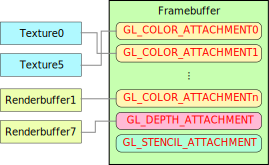
\includegraphics[width=10cm,keepaspectratio]{pics/framebuffer/framebuffer.pdf}
  \end{figure}
\end{frame}


\begin{frame}
\frametitle{Použití FBO}
    \begin{enumerate}
        \item{Získání jména FBO.}
        \item{Aktivování FBO.}
        \item{Připojení textur/renderbufferů k attachmentům.}
        \item{Nastavení seznamu attachmentů.}
        \item{Deaktivace FBO.}
        \item{...}
        \item{Aktivování FBO.}
        \item{Vykreslení scény.}
        \item{Deaktivace FBO.}
        \item{Zpracování vyrenderovaných textur.}
    \end{enumerate}
\end{frame}

\begin{frame}[fragile]
\frametitle{Vytvoření/uvolnění FBO identifikátorů}
  \begin{itemize}
    \item{
    Vytvoření VBO identifikátorů:
    {\scriptsize
    \mint[frame=lines]{c++}|void glCreateFramebuffers(GLsizei n,GLuint * buffers);|
    }}
    \item{
    Uvolnění VBO identifikátorů:
    {\scriptsize
    \mint[frame=lines]{c++}|void glDeleteFramebuffers(GLsizei n,GLuint * buffers);|
    }}
  \end{itemize}
\end{frame}

\begin{frame}[fragile]
\frametitle{Ověření stavu FBO}
  \begin{itemize}
    \item{
    Pro ověření stavu FBO použijeme tuto funkci
    {\scriptsize
    \mint[frame=lines]{c++}|GLenum glCheckNamedFramebufferStatus(GLuint fbo,GLenum target);|
    }}
    \item{
    Pokud funkce vraci {\color{red} GL\_FRAMEBUFFER\_COMPLETE} je vše v pořádku.
    }
  \end{itemize}
\end{frame}


\begin{frame}[fragile]
\frametitle{Aktivování/deaktivování FBO}
  \begin{itemize}
    \item{
    Aktivování/deaktivování FBO:
    {\scriptsize
    \mint[frame=lines]{c++}|void glBindFramebuffer(GLenum target,GLuint framebuffer);|
    }
    \begin{description}
    \item[target] GL\_FRAMEBUFFER stejný buffer pro čtení i zápis, GL\_READ\_FRAMEBUFFER, GL\_DRAW\_FRAMEBUFFER.
    \item[framebuffer] Jméno FBO získané {\color{blue} glGenFramebuffers}.
    Pokud nastaveno na 0 deaktivuje buffer.
    \end{description}
    }
  \end{itemize}
\end{frame}

\begin{frame}[fragile]
\frametitle{Připojení textur}
  \begin{itemize}
    \item{
    Attachment představuje jeden podbuffer FBO - například hloubkový buffer.
    Připojení textur k attachmentům:
    {\scriptsize
    \begin{minted}[frame=lines]{c++}
    void glNamedFramebufferTexture(GLuint fbo,GLenum attachment,
      GLuint texture,GLint level);
    \end{minted}
    }
    \begin{description}
    \item[fbo] framebuffer
    \item[attachment] Které informace budeme zapisovat do textury.
    GL\_DEPTH\_ATTACHMENT - hloubkový buffer.
    GL\_STENCIL\_ATTACHMENT - stencil buffer.
    GL\_COLOR\_BUFFERx - barva, nebo jiná informace.
    Specifikováno pomocí fragment shaderu (layout).
    \item[texture] Identifikátor textury.
    \item[level] Stupeň mipmappingu.
    \end{description}
    }
    \item Layered rendering
    {\scriptsize
    \begin{minted}[frame=lines]{c++}
    void glNamedFramebufferTextureLayer(GLuint fbo,GLenum attachment,
      GLuint texture,GLint level,GLint layer);
    \end{minted}
    }
  \end{itemize}
\end{frame}

\begin{frame}[fragile]
\frametitle{Nastavení seznamu attachmentů (MRT)}
  \begin{itemize}
    \item{
    Nastavením seznamu attachmentů definujeme, do kterých barevných bufferů se bude kreslit.
    {\scriptsize
    \begin{minted}[frame=lines]{c++}
    void glNamedFramebufferDrawBuffers(GLuint id,GLsizei n,const GLenum * bufs);
    \end{minted}
    }
    \begin{description}
    \item[id] framebuffer
    \item[n] Počet bufferů, do kterých budeme kreslit.
    \item[bufs] Seznam GL\_COLOR\_BUFFERx.
    Pořadí specifikuje, ke kterému layout ve fragment shaderu bude buffer navázán.
    \end{description}
    }
  \end{itemize}
\end{frame}

\begin{frame}[fragile]
\frametitle{Kompletní příklad}
    Do textur budeme vykreslovat barvu, normálu a hloubku.
    Fragment shader:
    {\scriptsize
    \begin{minted}[frame=lines]{glsl}
#version 430
layout(location=0)out vec4 fragColor;//jeden vystup - drawbuffer0
layout(location=1)out vec3 fragNormal;//druhy vystup - drawbuffer1
//...
void main(){
  //...
  fragColor=vec4(fCol,1);//zapis barvy
  fragNormal=(fNor+1)/2;//zapis normaly
}
    \end{minted}
    }
\end{frame}

\begin{frame}[fragile]
\frametitle{Kompletní příklad}
    Aplikace - inicializace:
    {\tiny
    \begin{minted}[frame=lines]{c++}
glTexImage2D(GL_TEXTURE_2D,0,GL_RGBA8F,WIDTH,HEIGHT,0,GL_RGBA,
  GL_UNSIGNED_BYTE,NULL);//alokujeme misto
//...
glTexImage2D(GL_TEXTURE_2D,0,GL_RGB32F,WIDTH,HEIGHT,0,GL_RGBA,
  GL_UNSIGNED_BYTE,NULL);//alokujeme misto
//...
glTexImage2D(GL_TEXTURE_2D,0,GL_DEPTH_COMPONENT24,
  WIDTH,HEIGHT,0,GL_DEPTH_COMPONENT,GL_UNSIGNED_BYTE,NULL);

glCreateFramebuffers(1,&fbo);//vygenerujeme nazev pro FBO

//navazani textur
glNamedFramebufferTexture(fbo,GL_DEPTH_ATTACHMENT,
  tDepth,0);//navazeme texturu pro hloubku
glNamedFramebufferTexture(fbo,GL_COLOR_ATTACHMENT3,
  tColor,0);//navazeme texturu pro barvu
glNamedFramebufferTexture(GL_FRAMEBUFFER,GL_COLOR_ATTACHMENT5,
  tNormal,0);//navazeme texturu pro normalu

GLenum drawBuffers[]={
  GL_COLOR_ATTACHMENT3,//layout(location=0)out vec4 fragColor;
  GL_COLOR_ATTACHMENT5//layout(location=1)out vec3 fragNormal;
};
glNamedFramebufferDrawBuffers(fbo,2,drawBuffers);//nastavime seznam cilu

if(glCheckNamedFramebufferStatus(fbo,GL_FRAMEBUFFER)!=GL_FRAMEBUFFER_COMPLETE)
  std::cerr<<"chyba\n";
glBindFramebuffer(GL_FRAMEBUFFER,0);
    \end{minted}
    }
\end{frame}

\begin{frame}[fragile]
\frametitle{Kompletní příklad}
    Aplikace - kresleni:
    {\scriptsize
    \begin{minted}[frame=lines]{c++}
glBindFramebuffer(GL_FRAMEBUFFER,FBO);//aktivujeme FBO
glDrawArrays(...);
glBindFramebuffer(GL_FRAMEBUFFER,0);//deaktivovani FBO
    \end{minted}
    }
\end{frame}

\setbeamercolor{background canvas}{bg=fitblue}
\begin{frame}
\frametitle{Hierarchický depth buffer}
\begin{center}
\Huge {\color{white}Hierarchický depth buffer}
\end{center}
\end{frame}
\setbeamercolor{background canvas}{bg=white}

\begin{frame}[fragile]
\frametitle{Kompletní příklad tvorba hier. z-bufferu}
		GLSL - CreateHierarchy:
		{\tiny
		\begin{minted}[frame=lines]{glsl}
//vertex shader////////////////////////////////////////////////////////////
#version 430
void main(){
  gl_Position=vec4(0);
}
//geometry shader//////////////////////////////////////////////////////////
#version 430
layout(points)in;
layout(triangle_strip,max_vertices=4)out;
void main(){
  gl_Position=vec4(-1,-1,0,1);EmitVertex();
  gl_Position=vec4(+1,-1,0,1);EmitVertex();
  gl_Position=vec4(-1,+1,0,1);EmitVertex();
  gl_Position=vec4(+1,+1,0,1);EmitVertex();
}
//fragment shader///////////////////////////////////////////////////////////
#version 430
layout(binding=0)uniform sampler2D Last;//last mipmap
layout(location=0)out vec2 fDepth;//output depth
ivec2 Coord=ivec2(gl_FragCoord.xy);//coordinates
void main(void){
  vec2 A=texelFetch(Last,Coord*2+ivec2(0,0),0).xy;
  vec2 B=texelFetch(Last,Coord*2+ivec2(1,0),0).xy;
  vec2 C=texelFetch(Last,Coord*2+ivec2(0,1),0).xy;
  vec2 D=texelFetch(Last,Coord*2+ivec2(1,1),0).xy;
  fDepth=vec2(min(min(A.x,B.x),min(C.x,D.x)),max(max(A.y,B.y),max(C.y,D.y)));
}
		\end{minted}
		}
\end{frame}

\begin{frame}[fragile]
\frametitle{Kompletní příklad tvorba hier. z-bufferu}
		Aplikace - inicializace:
		{\scriptsize
		\begin{minted}[frame=lines]{c++}
glGenTextures(1,&Depth);
//textura obsahujici minimalni a maximalni hloubku
glBindTexture(GL_TEXTURE_2D,Depth);
glTexParameteri(GL_TEXTURE_2D,GL_TEXTURE_MAG_FILTER,GL_NEAREST);
glTexParameteri(GL_TEXTURE_2D,GL_TEXTURE_MIN_FILTER,GL_NEAREST_MIPMAP_NEAREST);
int Size=WSize;
int Level=0;
while(Size>0){//smycka pres levely
  glTexImage2D(GL_TEXTURE_2D,Level++,GL_RG32F,Size,Size,0,GL_RG,
    GL_FLOAT,NULL);//alokace vrstvy
  Size/=2;
}
//render buffer s hloubkou
glCreateRenderbuffers(1,&RBO_Depth);
glNamedRenderbufferStorage(RBO_Depth,GL_DEPTH_COMPONENT,WSize,WSize);

glCreateFramebuffers(1,&FBO);//vygenerujeme nazev pro FBO
		\end{minted}
		}
\end{frame}


\begin{frame}[fragile]
\frametitle{Kompletní příklad tvorba hier. z-bufferu}
		Aplikace - render2 - tvorba hierarchie:
		{\tiny
		\begin{minted}[frame=lines]{c++}
glUseProgram(CreateHierarchy);
int Level=1;
int ActSize=WSize/2;
glBindFramebuffer(GL_FRAMEBUFFER,HFBO);//bind framebuffer
glActiveTexture(GL_TEXTURE0);//activate tex. unit 0
glBindTextureUnit(0,Depth);//bind depth texture to tex. unit 0
while(ActSize>0){//while there are
  glViewport(0,0,ActSize,ActSize);//set viewport
  glTexParameteri(GL_TEXTURE_2D,GL_TEXTURE_BASE_LEVEL,Level-1);//starting mipmap level
  glTexParameteri(GL_TEXTURE_2D,GL_TEXTURE_MAX_LEVEL,Level-1);//max mipmap level
  glNamedFramebufferTexture(FBO,GL_COLOR_ATTACHMENT0,Depth,Level);
  GLenum DrawBuffers[]={GL_COLOR_ATTACHMENT0};
  glNamedFramebufferDrawBuffers(1,DrawBuffers);
  glDrawArrays(GL_POINTS,0,1);
  Level++;//increment level of mipmap
  ActSize/=2;//actual size of mipmap
}
glBindFramebuffer(GL_FRAMEBUFFER,0);//unbind framebffer
glTexParameteri(GL_TEXTURE_2D, GL_TEXTURE_BASE_LEVEL, 0);//starting mipmap level
glTexParameteri(GL_TEXTURE_2D, GL_TEXTURE_MAX_LEVEL, Level-1);//max mipmap level
glViewport(0,0,WSize,WSize);//reset viewport
		\end{minted}
		}
\end{frame}


\setbeamercolor{background canvas}{bg=fitblue}
\begin{frame}
\frametitle{Layered Rendering}
\begin{center}
\Huge {\color{white}Layered Rendering}
\end{center}
\end{frame}
\setbeamercolor{background canvas}{bg=white}

\begin{frame}[fragile]
\frametitle{Layered rendering, cube map}
Cube map rendering - CPU
{\tiny
\begin{minted}[frame=lines]{c++}
GLuint cubeMap;
glCreateTextures(GL_TETURE_CUBE_MAP,1,&cubeMap);
for(size_t i=0;i<6;++i)
  glTextureImage2DEXT(cubeMap,GL_TEXTURE_CUBE_MAP_POSITIVE_X+i,0,
    GL_RGBA8,width,height,0,GL_RGBA,GL_UNSIGNED_BYTE,nullptr);
//it will attach all six sides of cube map
glNamedFramebufferTexture(cubeMap,GL_COLOR_ATTACHMENT0,cubeMap,0);
\end{minted}
}
\end{frame}

\begin{frame}[fragile]
\frametitle{Layered rendering, cube map}
Cube map rendering - Vertex Shader
{\tiny
\begin{minted}[frame=lines]{glsl}
layout(location=0)in vec3 position;
uniform float near = 0.1;
uniform float far  = 1000;
uniform vec4 lightPosition = vec4(0,0,0,1);
out int vInstanceID;
void main(){
  const mat4 views[6] = {
    mat4(vec4(+0,+0,-1,0), vec4(+0,-1,+0,0), vec4(-1,+0,+0,0), vec4(0,0,0,1)),
    mat4(vec4(+0,+0,+1,0), vec4(+0,-1,+0,0), vec4(+1,+0,+0,0), vec4(0,0,0,1)),
    mat4(vec4(+1,+0,+0,0), vec4(+0,+0,-1,0), vec4(+0,+1,+0,0), vec4(0,0,0,1)),
    mat4(vec4(+1,+0,+0,0), vec4(+0,+0,+1,0), vec4(+0,-1,+0,0), vec4(0,0,0,1)),
    mat4(vec4(+1,+0,+0,0), vec4(+0,-1,+0,0), vec4(+0,+0,-1,0), vec4(0,0,0,1)),
    mat4(vec4(-1,+0,+0,0), vec4(+0,-1,+0,0), vec4(+0,+0,+1,0), vec4(0,0,0,1))
  };

  mat4 projection = mat4(
    vec4(1,0,0,0),
    vec4(0,1,0,0),
    vec4(0,0,-(far+near)/(far-near),-1),
    vec4(0,0,-2*far*near/(far-near),0));
  gl_Position = projection*views[gl_InstanceID]*vec4(position-lightPosition.xyz,1);
  vInstanceID = gl_InstanceID;
}
\end{minted}
}
\end{frame}


\begin{frame}[fragile]
\frametitle{Layered rendering, cube map}
Cube map rendering - Geometry shader
{\tiny
\begin{minted}[frame=lines]{glsl}
layout(triangles)in;
layout(triangle_strip,max_vertices=3)out;
in int vInstanceID[];
void main(){
  gl_Layer = vInstanceID[0];
  gl_Position = gl_in[0].gl_Position;EmitVertex();
  gl_Position = gl_in[1].gl_Position;EmitVertex();
  gl_Position = gl_in[2].gl_Position;EmitVertex();
  EndPrimitive();
}
\end{minted}
}
\end{frame}


